%% LaTeX-Beamer template for KIT design
%% by Erik Burger, Christian Hammer
%% title picture by Klaus Krogmann
%%
%% version 2.1
%%
%% mostly compatible to KIT corporate design v2.0
%% http://intranet.kit.edu/gestaltungsrichtlinien.php
%%
%% Problems, bugs and comments to
%% burger@kit.edu

\documentclass[18pt]{beamer}

%% SLIDE FORMAT

% use 'beamerthemekit' for standard 4:3 ratio
% for widescreen slides (16:9), use 'beamerthemekitwide'
% for widescreen slide without sidebar use 'beamerthemekitwidenosidebar'
\usepackage{pgf}
\usepackage{templates/beamerthemekit}
%\usepackage{templates/beamerthemekitwide}
%\usepackage{templates/beamerthemekitwidenosidebar}

% use this to disable the latex beamer navigation symbols
\beamertemplatenavigationsymbolsempty


%% TITLE PICTURE

% if a custom picture is to be used on the title page, copy it into the 'logos'
% directory, in the line below, replace 'mypicture' with the 
% filename (without extension) and uncomment the following line
% (picture proportions: 63 : 20 for standard, 169 : 40 for wide
% *.eps format if you use latex+dvips+ps2pdf, 
% *.jpg/*.png/*.pdf if you use pdflatex)

\titleimage{GoodWillHunting}

%% TITLE LOGO

% for a custom logo on the front page, copy your file into the 'logos'
% directory, insert the filename in the line below and uncomment it

\titlelogo{H5P-Logo}

% (*.eps format if you use latex+dvips+ps2pdf,
% *.jpg/*.png/*.pdf if you use pdflatex)

%% TikZ INTEGRATION

% use these packages for PCM symbols and UML classes
% \usepackage{templates/tikzkit}
% \usepackage{templates/tikzuml}

% the presentation starts here

\title[IMP]{IMP}
\subtitle{Informatik, Mathematik, Physik}
\author{Malte Vo\ss}

\institute{Abteilung für Didaktik der Mathematik}

\date{5. Februar 2020}

% Bibliography

\usepackage{babelbib}
\bibliographystyle{babplain-lf}
\usepackage{tikz}
\tikzstyle{vertex}=[circle, draw, inner sep=0pt, minimum size=6pt]
\usetikzlibrary[topaths]

\begin{document}

% change the following line to "ngerman" for German style date and logos
\selectlanguage{ngerman}

%title page
\begin{frame}
\titlepage
\end{frame}

\section*{Feedback}

\begin{frame}{Gesamtbewertung}
    \begin{figure}[]
        \centering
        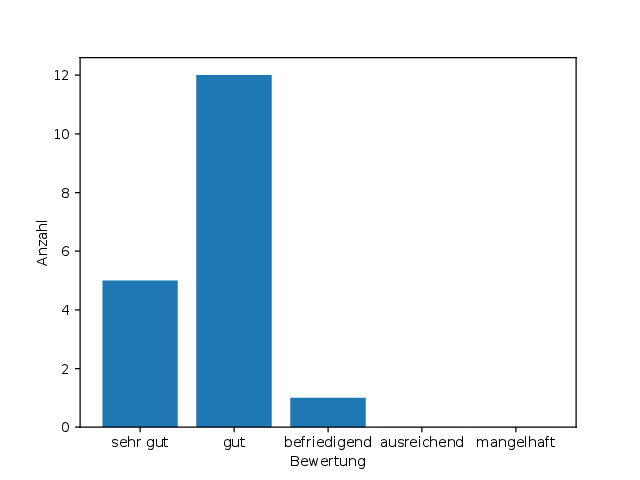
\includegraphics[keepaspectratio,width=0.69\textwidth]{figures/noten.png}
        \caption{Gesamtbewertung}
    \end{figure}
\end{frame}

\begin{frame}{Medieneinsatz}
    \begin{itemize}[<+->]
        \item Folien
        \begin{itemize}
            \item schön
            \item gute Animationen
        \end{itemize}
        \item Tafel 
        \begin{itemize}
            \item chaotisch, gequetscht, zu klein
            \item anschauliche Beispiele
            \item gute Ergänzung
        \end{itemize}
        \item abwechslungsreich
        \item flüssige Übergänge
        \item anderer Beamer wegen Ton
    \end{itemize}
\end{frame}

\begin{frame}{Vortragsweise}
    \begin{columns}
        \begin{column}{0.5\textwidth}
            \textbf{Zu verbessern:}
            \begin{itemize}
                \item zu viel Kontakt zu Folien
                \item \glqq Okay\grqq
                \item lebendiger, dynamischer, enthusiastischer
                \item sicherer, selbstbewusster
            \end{itemize}
        \end{column}
        \pause
        \begin{column}{0.5\textwidth}
            \textbf{Gut:}
            \begin{itemize}
                \item frei
                \item ruhig
                \item deutlich und klar
                \item sicheres Auftreten
            \end{itemize}
        \end{column}
    \end{columns}

    \pause
    \vspace{1cm}
    \textbf{Sonstiges:}
    \begin{itemize}[<+->]
        \item manche Inhalte (z.B. Möbiusband, Euler-Characteristik) genauer erklären
        \item mehr Bezug zur Schule
        \item mehr Überblick über IMP
        \item mehr als Graphen
        \item Zeitmanagement
    \end{itemize}
\end{frame}

%table of contents
\begin{frame}{Gliederung}
\tableofcontents
\end{frame}

\section{Flipped Classroom}
\begin{frame}{Flipped Classroom}
    \begin{itemize}[<+->]
        \item auch bekannt als Inverted Classroom, umgedrehter Unterricht
        \item Lehrsequenzen werden zu Hause durchgeführt
        \item Übungen im Unterricht (Coaching)
    \end{itemize}
\end{frame}

\begin{frame}{Flipped Classroom - Vergleich}
    \centering
    \begin{tabular}{cc}
        Klassischer Unterricht      & Flipped Classroom \\
        \hline
        \pause
        lehrergelenkt               & Schüler selbstbestimmt\\
        \pause
        Tempo des Lehrers           & eigenes Tempo \\
        \pause
        Pädagoge anwesend           & Schüler allein \\
        \pause
        meist analog                & digital \\
        \pause 
        Lernklima der Klasse        & ? \\
        \pause
        direkte Rückmeldung         & ? \\
        \pause
        beschränkt verfügbar        & im Internet \\
    \end{tabular}

    \vfill
    
    \begin{itemize}
        \item[$\Rightarrow$] Herausforderungen bei der Umsetzung
        \item[$\Rightarrow$] Anforderungen an das Tool
    \end{itemize}

    \begin{flushright}
        \cite{Schmidt}
    \end{flushright}
\end{frame}

\section{H5P}
\begin{frame}{H5P}    
    \begin{itemize}
        \item ist Open Source
        \item Technologie: HTML5
        \item wird als Erweiterung für ILIAS und Moodle angeboten
        \item viele Anwendungstypen, u.a. \textbf{Interactive Video}
    \end{itemize}
    \pause
    \vfill
    \huge LIVE-Demo

    \normalsize 
    \url{https://scc-ilias-plugins.scc.kit.edu/}

    \url{https://www.youtube.com/watch?v=-9OUyo8NFZg}
\end{frame}

\section{Praktikum}
\begin{frame}{Praktikum - Aufgabe}
    In Gruppen á 2 oder 3 Personen
    \begin{enumerate}[<+->]
        \item Dreht ein Lehr-Video zu einem selbstgewählten Thema
            \begin{itemize}
                \item Beispiele: euer Vortragsthema, euer Werkzeug, eine Vorlesung, Umkreismittelpunkt \dots
                \item etwa 2-3 Minuten
                \item ScreenCapture (Jing), Präsentation, Aufschrieb, \dots
                \item mögliche Aufgaben überlegen
                \item etwa 25 Minuten Zeit, freie Raumwahl
                \item auch möglich: fremde Materialien (YouTube, GeoGebra)
            \end{itemize}
        \item Ladet das Video in ILIAS hoch und fügt interaktive Elemente hinzu.
            \begin{itemize}
                \item \url{https://scc-ilias-plugins.scc.kit.edu/}
                \item Bibliothek: Interactive Video
            \end{itemize}
        \item Präsentiert euer Video $\ddot{\smile}$
    \end{enumerate}
    \vfill

    \pause
    Bei Fragen stehe ich gerne zu Verfügung.
\end{frame}

\begin{frame}{Diskussion}
    \begin{itemize}[<+->]
        \item Flipped Classroom allgemein -- Vor- und Nachteile
        \item Aufwand zum Erzeugen von Videos vs. vorhandenes Material nutzen
        \item Bedienbarkeit von H5P
    \end{itemize}
\end{frame}

    

    \appendix
    \beginbackup

    \begin{frame}[allowframebreaks]{Quellen}
    \bibliography{references}
    \end{frame}

    \backupend

    \begin{frame}{Vielen Dank für die Aufmerksamkeit!}
        \begin{figure}[]
            \centering
            
\includegraphics[keepaspectratio, width=0.5\textwidth]{figures/qr_pract.png}
            \caption{QR-Code zu \url{http://invote.de/53350}}
        \end{figure}
    \end{frame}
\end{document}
